\model{Computer Architecture}
\label{CSP/architecture}

Here is the 8-bit machine described in Appendix~C of Brookshear and Brylow (2015):

\begin{center}
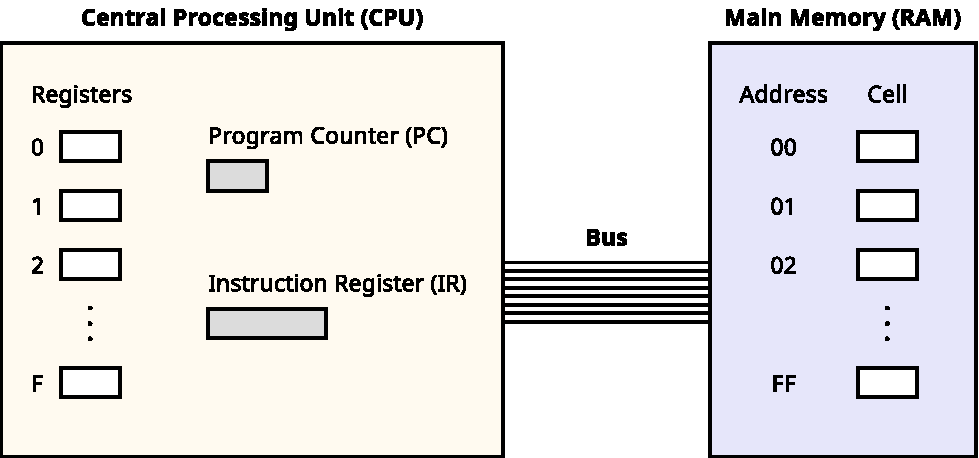
\includegraphics[width=0.8\linewidth]{CSP/cpu-bus-ram.pdf}
\end{center}


\quest{12 min}


\Q What are the three main components in the diagram?
Based on its name, what do you think each hardware component does?

\begin{answer}
The CPU is ``the brain'' of the computer that performs calculations and makes decisions.
The RAM is where ``working memory'' is stored.
The Bus connects the CPU and RAM together.
\end{answer}


\Q How many registers does the CPU have? How many memory cells are in RAM?
%Why do you think there are more memory cells than registers?

\begin{answer}[3em]
16 registers (0--F) and 256 memory cells (00--FF).
\end{answer}


\Q The CPU has circuits for adding the contents of two registers; think of registers as the ``pins'' in last week's lab.
What is the largest number this machine can add without overflowing?

\begin{answer}
Because the machine has eight bits, the largest number is 0xFF or 255.
\end{answer}


\Q Common tasks the CPU performs include \emph{loading} data from a memory cell into a register and \emph{storing} data from a register into a memory cell.
Describe what the CPU would need to do in order to add twenty numbers stored in memory.

\begin{answer}[7em]
The CPU would need to use two registers: one for a running total, and one to load data from memory.
Start by setting the total register to zero.
For each number, load it into the other register, and then add it to the total.
\end{answer}
